\chapter*{}
    \begin{center}
    \textbf{LEMBAR PENGESAHAN}\\
    \textbf{TUGAS AKHIR}\\

	\vspace*{1 cm}

    \textbf{\Judul}\\
    \textit{\textbf{\JudulInggris}}\\
    
	\vspace*{1 cm}
    
    \bo{
    Telah disetujui dan disahkan sebagai Tugas Akhir\\
    		\program\\
        	\fakultas\\
        	Telkom University\\
        	Bandung \\
    }
    
	\vspace*{1.0cm}    
    
    Disusun oleh\\
    	\vspace*{0.5 cm} 
    \bo{\penulis} \\
    \bo{\nim} \\

    \vspace*{1.0cm}
    \textbf{Bandung, \tanggalPengesahan\\
    Menyetujui,}
    \end{center}
    
    \begin{tabular}{>{\centering\arraybackslash} p{0.3\paperwidth} >{\centering\arraybackslash} p{0.3\paperwidth}}\\
    Pembimbing I & Pembimbing II \\ [3 cm]
    \uline{\pembimbingSatu} & \uline{\pembimbingDua} \\
    \nikSatu & \nikDua
    \end{tabular}
 
%    
%\hspace*{5in}
%\vspace*{-5in}
%\begin{figure}[t!]
%\centering
%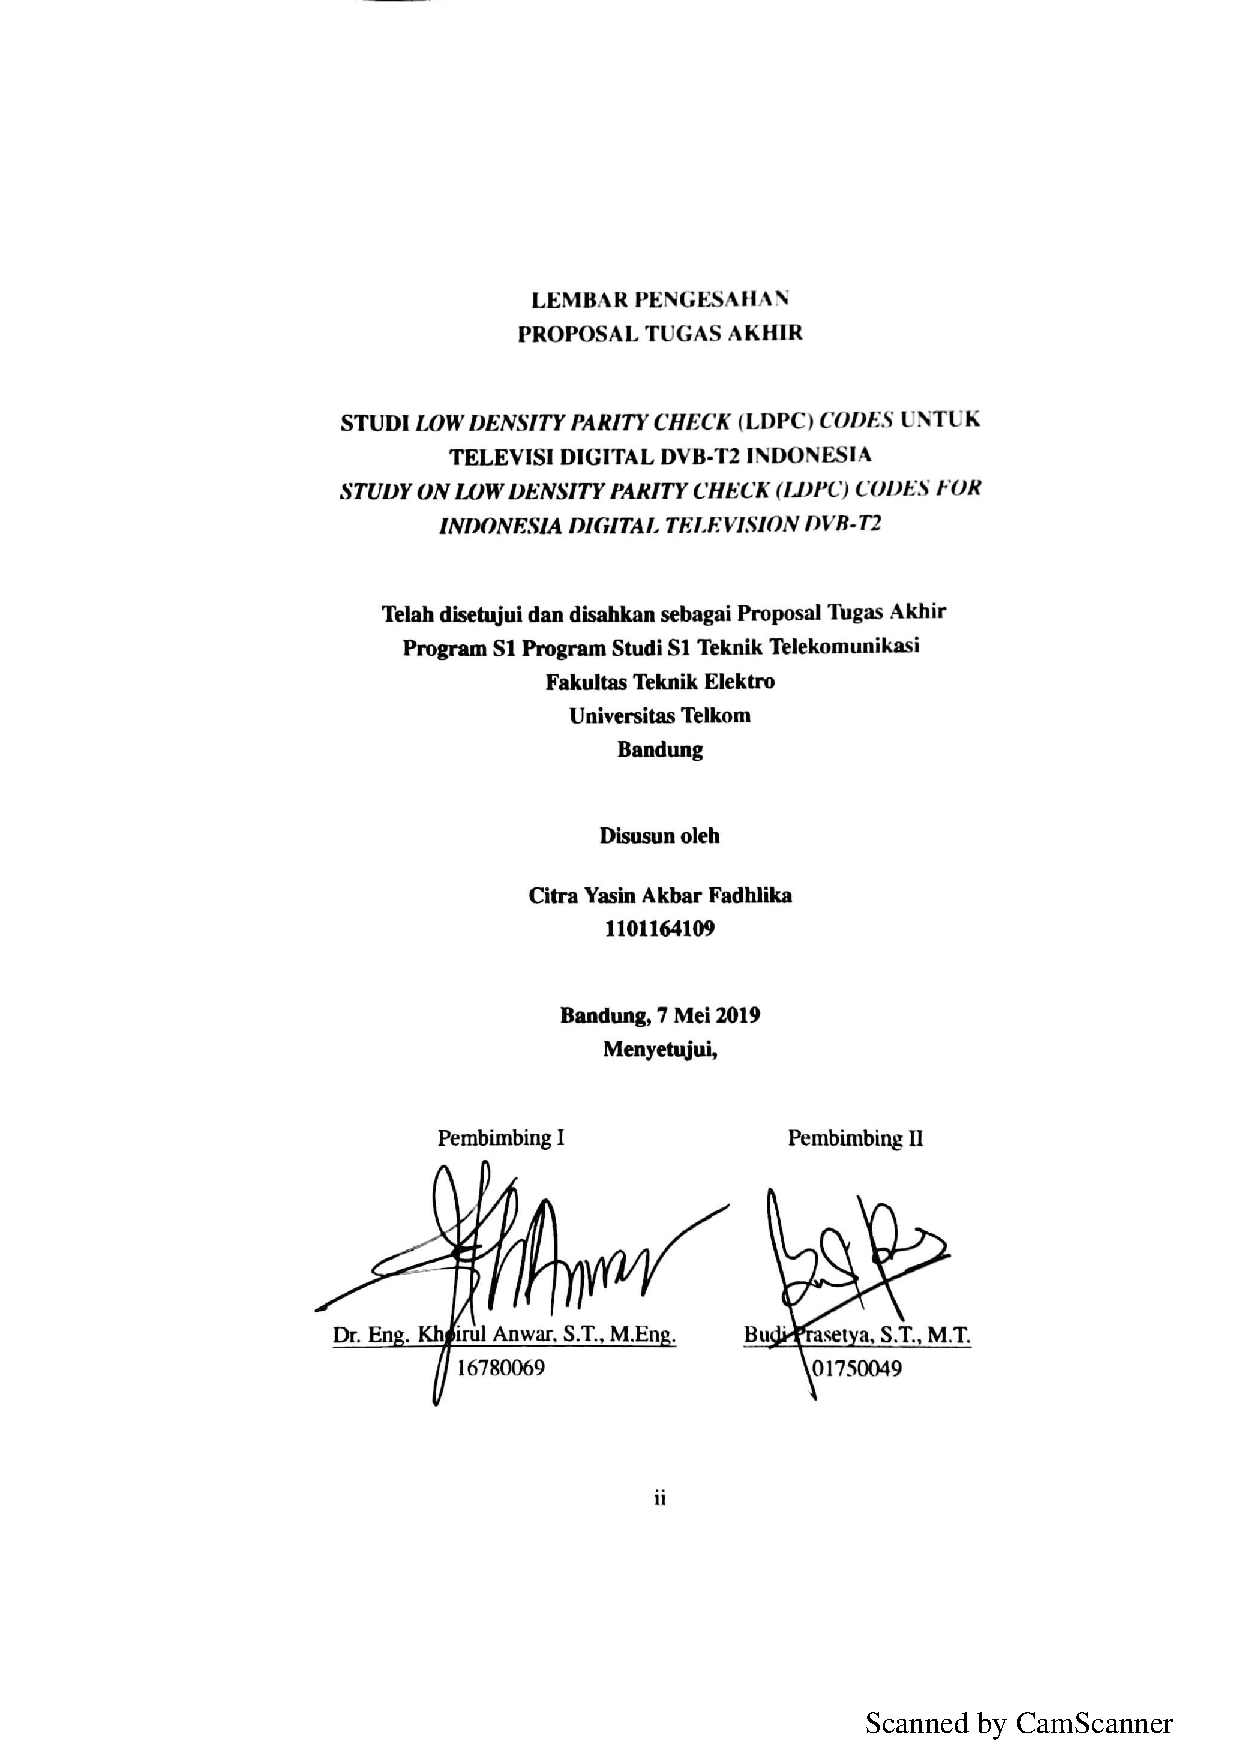
\includepdf[pages=-,pagecommand={},scale=1.18]{pengesah.pdf}
%	
%\end{figure}
%\thispagestyle{empty}